% Chapter Template

\chapter{Project requirements} % Main chapter title

\label{Chapter4} % Change X to a consecutive number; for referencing this chapter elsewhere, use \ref{ChapterX}
\section{Hybrid Desktop with Mixed Reality survey}
At the start of the project, a survey has been done to find the current requirements about AR/VR application among university students.
\\
\\
The survey involved the following questions: 1. Which way do you prefer to express your idea? 2. How do you usually revise your lecture notes? 3. If you don’t like physical materials, which are the possible reasons? 4. Would you want to have an electronic bookshelf to organize all your course materials? 5. Where do you prefer to study? 6. Do you love your current study habit? If not, why? Participates are able to access this questionnaire by surveyMonkey (an online survey tool)[11], and this web link is shared by Messager (A chat tool created by FaceBook). 
\\
\\
In October 11th 2016, 88 university students completed this survey. And the result(shown in Figure 4.1) indicates that although more people prefer to work with physical materials, most people work with electronic documents during their real study time. Participants think the reasons is physical materials are easy to lose and hard to organize, and the reason for their preference with electronic desktop is they can share their electronic copy easily and manage these documents on the cloud which provide wider and easier operation with documents. But the reason for their preference for physical materials are they are express their ideas easily and write something down on the notebook is convenient, they can write it down anywhere and anytime. 
\\
\\
Because of the fast development of portable device, more students prefer to go to lecture with their iPad and take notes with iPad as well. Laptop is heavy to carry and the human nature is they prefer light and convenient belongs. The paradox is when they study at home, they prefer to study with laptop. Because the undeniable fact is laptop is much more powerful and it provides larger screen which gives better user experience. Furthermore, 68.18\% students are not satisfied with their current study habit, and 78.3\% of these people think the main reason is they are lazy and need someone to remind them all the time, so this project decided to provide a AI servant which can be served as an assistant to remind students stay focused. And if there is an electronic bookshelf (document list) to help them organize materials, 90.91\% students are willing to have this application. 
\\
\\
In conclusion, the current study habits among university students have some problems and because of the fast development of internet, electronic materials became an inseparable part of university study. The university students need a workstation which can provide them the clearest structure of their materials, give them the easiest access to all their documents and it should be easy to carry and set up. Based on this survey, we can conclude that if we can figure these problems out, the future of Hybrid desktop is promising. Besides, different students in different major will have their special needs for the course. For example, mechanical students hope to see their models in a 3D way, data science students hope to visualize their data. By using Mixed reality technology, these dreams can come into reality.
\begin{figure}[h]
    \centering
	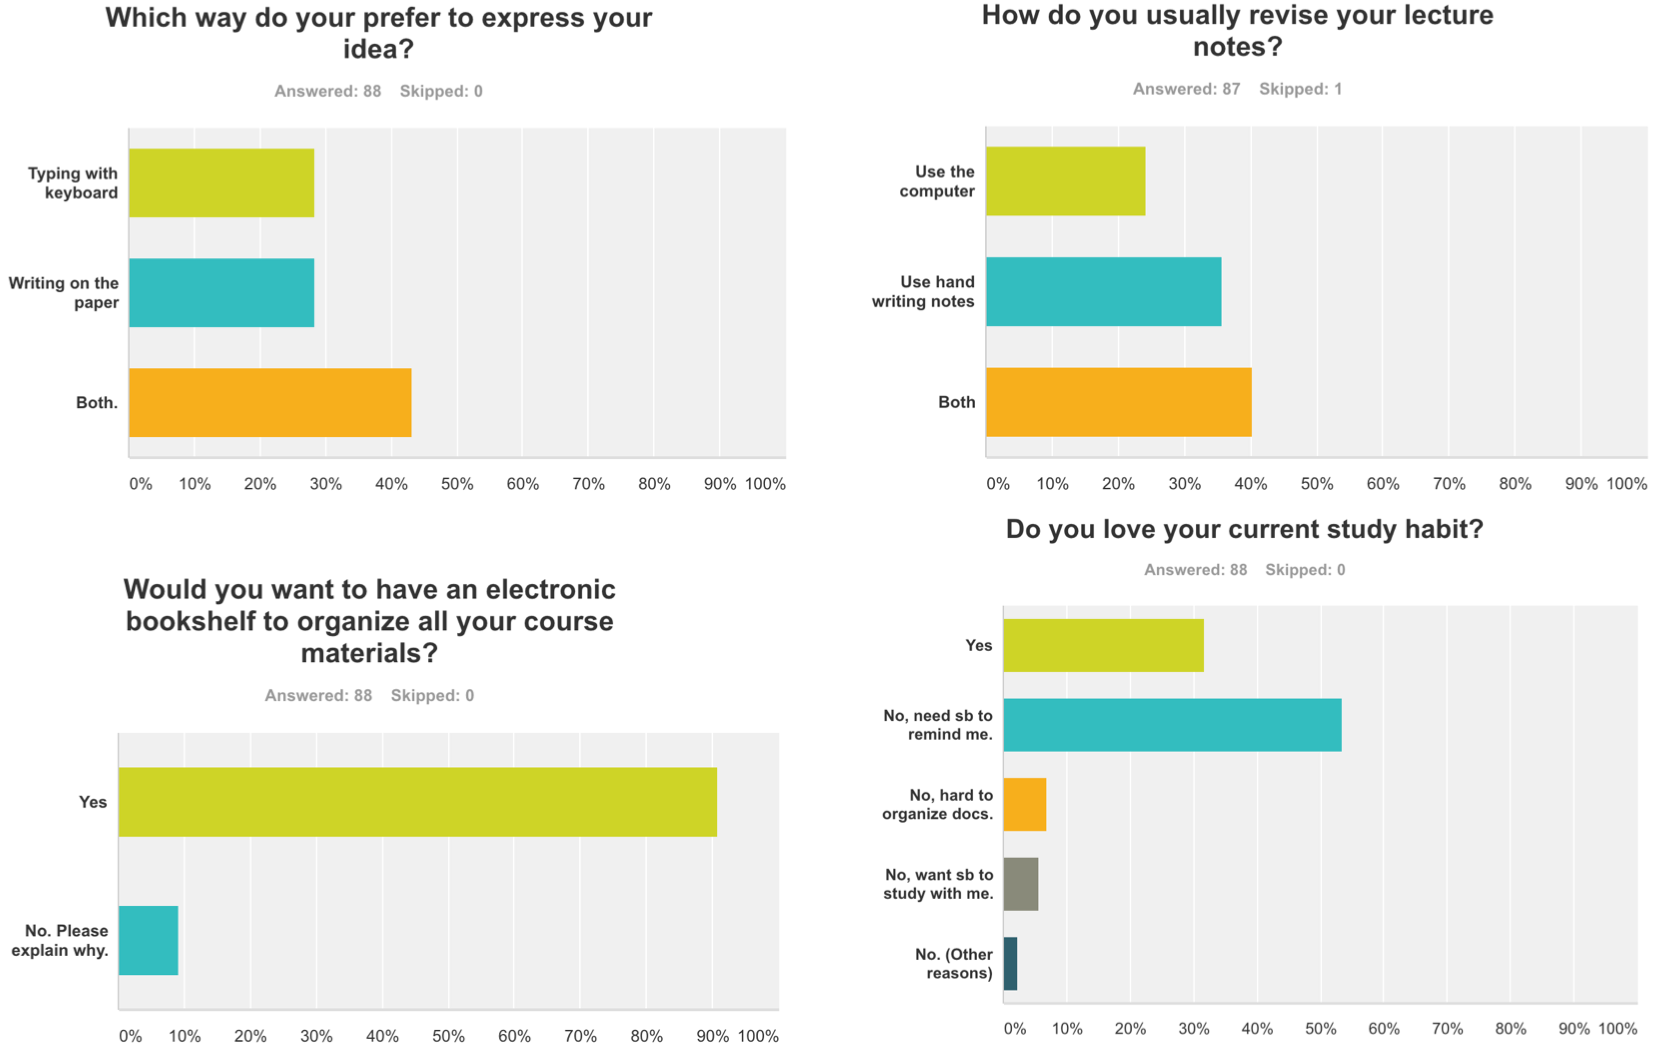
\includegraphics[width=\textwidth]{survey}
    \caption{Some survey results among 88 university students}
    \label{fig:mesh1}
\end{figure}

\section{Scenario}
Based on the background information and the survey, this project proposes the following scenario:
\\
\\
When students put their phone in the Google Cardboard or any other Cardboard they prefer, and wear their VR headset, by recognizing the “Hybrid desktop QR code”, all the digital objects like PDF/PPT reader, AI servant and bulletin board will display on the physical desktop.
\\
\\
AI servant is served as an office assistant which is a user interface that assisted users by the way of an interactive animated character. It is used to show users the status of imageTarget, their gestures recognition progress and give students the information of their hands to help them perform the targeted gestures accurately. And it can also be considered as the communication tool between the systems and devices. 
\\
\\
And bulletin board is going to show user’s daily tasks and some general information about weather and date. Users can create and manage their tasks through the hybrid desktop website. This website can also be used as a tool for electronic annotation. When the user is typing in the textfield in the annotation web page, their text will show on the electronic annotation box automatically. This hybrid desktop website is served as a platform to control any data which belongs to the users. 
\\
\\
There is a large PDF/PPT reader on the right side of the desktop. Students can view their module materials in this screen or they can switch the slides by clicking some buttons like moving to the next slide or move back to the previous slide and the relative module materials will display in the PDF/PPT reader. In order to change the size of the PDF reader, the users can do a clockwise gesture, and it stands for zooming out the PDF reader. The gesture of counterclockwise stands for zooming in the PDF reader. By performing gestures, the PDF reader should be able to change position as well. Once, the camera recognizes the marker, it will display all the digital objects, even if it loses the track of the image target. So, when the user moves their head, they do not need to worry about there may cause the mess of these digital objects.


\section{Proposed functionality}
\subsection{AR document list and PDF reader}
Document list is used for displaying all the available materials for students. And there will be an arrow which points to the displaying PDF, so students can check what module he/she is studying in a clear way. Besides, it enables user to select documents by hovering their hands above the switch button. One of the special functions is user can write down the code of the documents to display that material, and the code of documents should be the same name on the documents list. The selected PDF will be displayed in the PDF reader, and it will enable user to change the size of the reader, and switch slides. It should be better if the users are able to move the PDF reader.


\subsection{Bullet board}
Bulletin board is displayed in the most noticeable place, so the project aims to let it give students the information which they need to check most frequently. For example, the weather, date information, and their tasks. Students can manage these tasks by using the hybrid desktop website, and all the information presented on the bulletin board should be the latest one.


\subsection{Artificial Intelligence servant}
AI servant is used for managing and reminding user’s tasks and documents. The survey shows that most students are not satisfied with their study habits, so AI servant can be used to remind the students when they are not highly focusing on study. And it will add more fun to the desktop. It will also be an interface to tell students what gestures this application is recognizing and whether the imageTarget is trackable or not.

\subsection{Electronic annotation displaying system}
Users are able to make annotations for both electronic and physical materials, so these annotations need to be located accurately when the system retrieve the data. In hybrid desktop’s website, users can check their notes by category and choose which one to display in the virtual world. For better user experience, these electronic annotations should be able to move by the physical documents as well. So, these annotation is not positioned in the same place all the time.

\subsection{Hybrid Desktop Website}
This website is built for managing user’s data and taking annotations. This website breaks the barrier of devices. In this project, because these annotations are stored on web server, if users want to make annotations, they can use whatever they want. For example, they can use their phone, pad or even raspberry to get access to this website and make annotation. Besides, this website has a further section which is waiting for future implementation. Users are able to send message to the developer and tell them what new features they want, and what improvement they hope for.

\section{Platforms and Tools}
Based on the proposed functionalities, the project selects the following platforms and tools.
\subsection{Unity as developing platform}
Unity has introduced built-in support for certain AR/VR devices, and it is the most popular and powerful platform to build a AR/VR application. And Unity can be considered as the multiplatform game engine. With Unity, developers are able to get one-click deployment to the full range of mobile and VR devices. The current platform of this project is mobile devices, based on Unity, the project does not need to use Android Studio and Xcode at the same time to develop these two mobile applications. It can build and run on both Android and IOS. So, this project chooses Unity as the development platform.
 
\subsection{Leap Motion for supporting gestures}
The future of virtual reality is truly immersing yourself in the virtual world with your hands. Leap Motion[12] is the device that helps the developers to reach this goal. This device senses how user naturally moves their hands, and gets the hand information like location of user’s finger and recognizes some sample gestures (clockwise circle, swipe, and etc). The users are able to interact with those virtual objects just like they do in the real world. So, it is useful for deceiving users' sense that they are actually interacting with these real objects. Leap Motion is supported for VR headset like Oculus and Mac or other PCs. For better interaction with hybrid desktop, this project will take the advantages of LeapMotion and allow user’s specific gestures to control the digital objects.
\\
\\
To explore Leap Motion SDK with standard tracking to control PDF reader by using different gestures, and interaction with electronic documents. It needs socket communication to support the data transfer. Furthermore, it requires new function for using Leap Motion’s hand information to display and control virtual objects. 


\subsection{Software development Kit}
There are two competitive open source augmented reality SDK, ARToolKit[7] and Vuforia[8]. Compared with ARToolKit, the special functionality of Vuforia is Vuforia has virtual buttons which allows some touchable zones in the tracking image and enable interaction with the device. Besides, Vuforia can support more platforms like windows app, and also for MS HoloLens. Although the current implementation is with IOS, future development will be run on other AR devices like HoloLens and Meta2 which can provide a clear and wider view. Because of the wide spread and relatively cheap price of smart phone, running hybrid desktop on smart phone gives more opportunities for students to get involved in this new experience.
\\
\\
Besides, vuforia has four advantages of being a leading AR platform: 1. Unparalleled reliability which enable vuforia delivers best-in-class computer vision, and providing robust experiences in a large amount of environments. 2. Creative empowerment which offer developers the creative freedom. 3. Maximum reach which supports most leading platforms. 4. Advanced vision which enables developer to use the most common thing as the marker. Based on all the concerns and superiority, Vuforia SDK can be considered as a better choice for this project.

\subsection{Programming Languages}
Scripting is an essential component of the project. Because this project chooses Unity as the developing platform, and Unity is preferable for C\#. Considering about the maintainability and integrity, C\# is preferable for this project as well. Then listing out the possible problems this project needs to figure out and thinking about whether C\# is suitable for solving this problem.
\\
\\
The disadvantage of Vuforia is it cannot locate user’s finger and return the track of user’s finger. But when implementing with PDF reader like using some gesture to control the PDF reader, the track of user’s finger is an essential information. To solve this problem, Leap Motion is introduced to this project. Nevertheless, Leap Motion cannot support with iPhone. So, there should be another implementation with exchanging information between Leap Motion and iPhone. 
\\
\\
There are two good programing languages which support this problem, C++ and C\#. At first, I choose C++ API of Leap Motion instead of C\#. The reason is the functionality of API between these two languages have no difference. But Leap Motion C++ API is both recommended and supported for Xcode on macOS and Visual Studio on Windows, but Leap Motion C\# API is strongly recommended to use with Visual Studio on Windows. Later, some problems with the implementation of C++ occurs. C\# client in Unity is not the best choice of C++ server, and mono can solve the problem of developing C\# application on macOS. Mono[9] provides the necessary software to develop and run ECMA CLI, C\# and .NET client and server application on different platform. It perfectly solved the inconvenience of developing C\# application on MAC.

\subsection{Database selection}
For the selection of database. At first, MongoDB was chosen to be the database for this project. However, after weeks of exploring the data structure of the project, I decided to change the database to MYSQL. The reasons are as follow: 1. It requires complex multi-row transactions, and MongoDB is not a drop-in replacement for legacy application built around the relational data model and SQL. 2. In MYSQL, related information may be stored in separate tables, but associated through the use of joins. And data duplication is minimized which is suitable for this project. 
\\
\\
So, this project selects the MYSQL as the database, and it needs to implement data storage and interaction with MYSQL and Unity. These data can be user based tasks, and the electronic annotations should be stored in MYSQL database as well. When users are making electronic annotations, information will be updated to the MYSQL database simultaneously, and the annotation box in hybrid desktop will have a HTTP GET request to get the information and display that in the Unity project.
PHP files will be uploaded on the server, and it will be used to request data from MYSQL databased. So, by requesting these web pages, the bulletin board can get user’s detailed information which is more suitable and easier to implement.

